\appendix
\newpage
\section{Additional results reproducing the original paper}
\label{add_original}
\subsection{Adult Dataset}

\begin{table}[H]
\begin{threeparttable}
\centering

\begin{tabular}{lrrrrrrrr}
\toprule
 & \multicolumn{4}{c}{Known DS} & \multicolumn{4}{c}{Unknown DS} \\
 & NSF & Acc & FR & $\Delta$ Acc & NSF & Acc & FR & $\Delta$ Acc \\
\cmidrule(r){2-5} \cmidrule{6-9}
FairConst & n/a & 0.784 & 1.000 & -0.004 & n/a & 0.784 & 0.250 & -0.007 \\
RFLearn & n/a & \bfseries 0.786 & 1.000 & -0.000 & n/a & \bfseries 0.788 & 1.000 & 0.001 \\
Fairlearn & n/a & 0.750 & 0.500 & -0.002 & n/a & 0.752 & 0.500 & -0.008 \\
Quasi-SC & 0.240 & 0.765 & 0.105 & 0.029 & 0.000 & 0.785 & \bfseries 0.000 & 0.020 \\
Shifty & 0.480 & 0.756\tnote{1} & \bfseries 0.000 & 0.020 & 0.000 & 0.780\tnote{2} & \bfseries 0.000 & 0.020 \\
SC & 0.520 & 0.756 & \bfseries 0.000 & n/a & 0.000 & 0.781 & \bfseries 0.000 & 0.032 \\
\bottomrule
\end{tabular}
\begin{tablenotes}
\item[1] significantly worse than best model, $p<0.001$, $t=14.256$, $df=36$
\item[2] significantly worse than best model, $p<0.001$, $t=8.892$, $df=14$
\end{tablenotes}
\end{threeparttable}
\caption{Comparison between the models for the greatest sample size using the Disparate Parity fairness definition and Adult dataset. Shifty differs significantly from the best performing model, and fewer solutions are found.  \textit{DS} = Demographic Shift, \textit{NSF} = No Solution Found, \textit{Acc} = Accuracy, \textit{FR} = Failure Rate, $\Delta$ \textit{Acc} = Difference in accuracy between the largest and smallest sample size.}
\label{dp_adult}
\end{table}
\begin{table}[H]
\begin{threeparttable}
\centering
\begin{tabular}{lrrrrrrrr}
\toprule
 & \multicolumn{4}{c}{Known DS} & \multicolumn{4}{c}{Unknown DS} \\
 & NSF & Acc & FR & $\Delta$ Acc & NSF & Acc & FR & $\Delta$ Acc \\
\cmidrule(r){2-5} \cmidrule{6-9}
FairConst & n/a & 0.783 & 0.040 & -0.004 & n/a & 0.783 & \bfseries 0.000 & -0.007 \\
RFLearn & n/a & \bfseries 0.786 & 0.800 & -0.000 & n/a & 0.787 & 1.000 & -0.001 \\
Fairlearn & n/a & 0.783 & 0.220 & 0.004 & n/a & 0.784 & 0.125 & -0.000 \\
Quasi-SC & 0.080 & 0.781 & \bfseries 0.000 & 0.046 & 0.250 & 0.792 & \bfseries 0.000 & -0.003 \\
Shifty & 0.240 & 0.781\tnote{1} & \bfseries 0.000 & 0.044 & 0.750 & 0.757\tnote{2} & \bfseries 0.000 & 0.025 \\
SC & 0.280 & 0.776 & \bfseries 0.000 & n/a & 0.625 & \bfseries 0.825 & \bfseries 0.000 & n/a \\
\bottomrule
\end{tabular}
\begin{tablenotes}
\item[1] significantly worse than best model, $p=0.002$, $t=3.241$, $df=42$
\item[2] insufficient number of solutions to perform t-test
\end{tablenotes}
\end{threeparttable}
\caption{Comparison between the models for the greatest sample size using the Equalized Odds fairness definition and Adult dataset. When the Demographic Shift (\textit{DS}) is known, Shifty differs significantly from the best performing model.}
\label{eodds_adult}
\end{table}
\begin{table}[H]
\begin{threeparttable}
\centering
\begin{tabular}{lrrrrrrrr}
\toprule
 & \multicolumn{4}{c}{Known DS} & \multicolumn{4}{c}{Unknown DS} \\
 & NSF & Acc & FR & $\Delta$ Acc & NSF & Acc & FR & $\Delta$ Acc \\
\cmidrule(r){2-5} \cmidrule{6-9}
FairConst & n/a & 0.783 & \bfseries 0.000 & -0.005 & n/a & 0.803 & \bfseries 0.000 & -0.005 \\
RFLearn & n/a & \bfseries 0.786 & 0.440 & -0.001 & n/a & 0.787 & 1.000 & -0.018 \\
Fairlearn & n/a & 0.782 & 0.080 & 0.001 & n/a & \bfseries 0.852 & 0.062 & 0.016 \\
Quasi-SC & 0.160 & 0.783 & \bfseries 0.000 & 0.047 & 0.000 & 0.822 & \bfseries 0.000 & 0.096 \\
Shifty & 0.280 & 0.783\tnote{1} & \bfseries 0.000 & 0.056 & 1.000 & n/a\tnote{2} & n/a & n/a \\
SC & 0.440 & 0.782 & \bfseries 0.000 & 0.049 & 0.500 & 0.812 & \bfseries 0.000 & n/a \\
\bottomrule
\end{tabular}
\begin{tablenotes}
\item[1] not significantly different from best model, $p=0.166$, $t=1.410$, $df=41$
\item[2] insufficient number of solutions to perform t-test
\end{tablenotes}
\end{threeparttable}
\caption{Comparison between the models for the greatest sample size using the Equal Opportunity fairness definition and Adult dataset. When the \textit{DS} is known, Shifty does not differ significantly from the best performing model.}
\label{eopp_adult}
\end{table}
\begin{table}[H]
\begin{threeparttable}
\centering
\label{pe_adult}
\begin{tabular}{lrrrrrrrr}
\toprule
 & \multicolumn{4}{c}{Known DS} & \multicolumn{4}{c}{Unknown DS} \\
 & NSF & Acc & FR & $\Delta$ Acc & NSF & Acc & FR & $\Delta$ Acc \\
\cmidrule(r){2-5} \cmidrule{6-9}
FairConst & n/a & 0.783 & 0.520 & -0.002 & n/a & 0.792 & \bfseries 0.000 & 0.002 \\
RFLearn & n/a & \bfseries 0.786 & 1.000 & -0.000 & n/a & 0.788 & 1.000 & -0.000 \\
Fairlearn & n/a & 0.781 & 0.980 & 0.003 & n/a & 0.783 & 0.750 & -0.002 \\
Quasi-SC & 0.200 & 0.779 & \bfseries 0.000 & 0.046 & 0.000 & 0.789 & \bfseries 0.000 & 0.022 \\
Shifty & 0.520 & 0.776\tnote{1} & \bfseries 0.000 & 0.046 & 0.125 & 0.795\tnote{2} & \bfseries 0.000 & 0.031 \\
SC & 1.000 & n/a & n/a & n/a & 0.250 & \bfseries 0.815 & \bfseries 0.000 & n/a \\
\bottomrule
\end{tabular}
\begin{tablenotes}
\item[1] significantly worse than best model, $p<0.001$, $t=5.871$, $df=35$
\item[2] not significantly different from best model, $p=0.201$, $t=1.360$, $df=11$
\end{tablenotes}
\end{threeparttable}
\caption{Comparison between the models for the greatest sample size using the Predictive Equality fairness definition and Adult dataset. When the \textit{DS} is known, Shifty differs significantly from the best performing model. There is no significant difference when the \textit{DS} is unknown.}
\end{table}
\clearpage

\begin{figure*}[h!]
    \begin{subfigure}[b]{1\linewidth}
        \includegraphics[width=\textwidth]{img/charts/adult/fixed/iclr_adult_demographic_shift_sex_di.png}
        \caption{Disparate Impact}
    \end{subfigure} 
    \begin{subfigure}[b]{1\linewidth}
        \includegraphics[width=\textwidth]{img/charts/adult/fixed/iclr_adult_demographic_shift_sex_dp.png}
        \caption{Demographic Parity}
    \end{subfigure}
    \begin{subfigure}[b]{1\linewidth}
        \includegraphics[width=\textwidth]{img/charts/adult/fixed/iclr_adult_demographic_shift_sex_eo.png}
        \caption{Equal Opportunity}
    \end{subfigure} 
    \begin{subfigure}[b]{1\linewidth}
        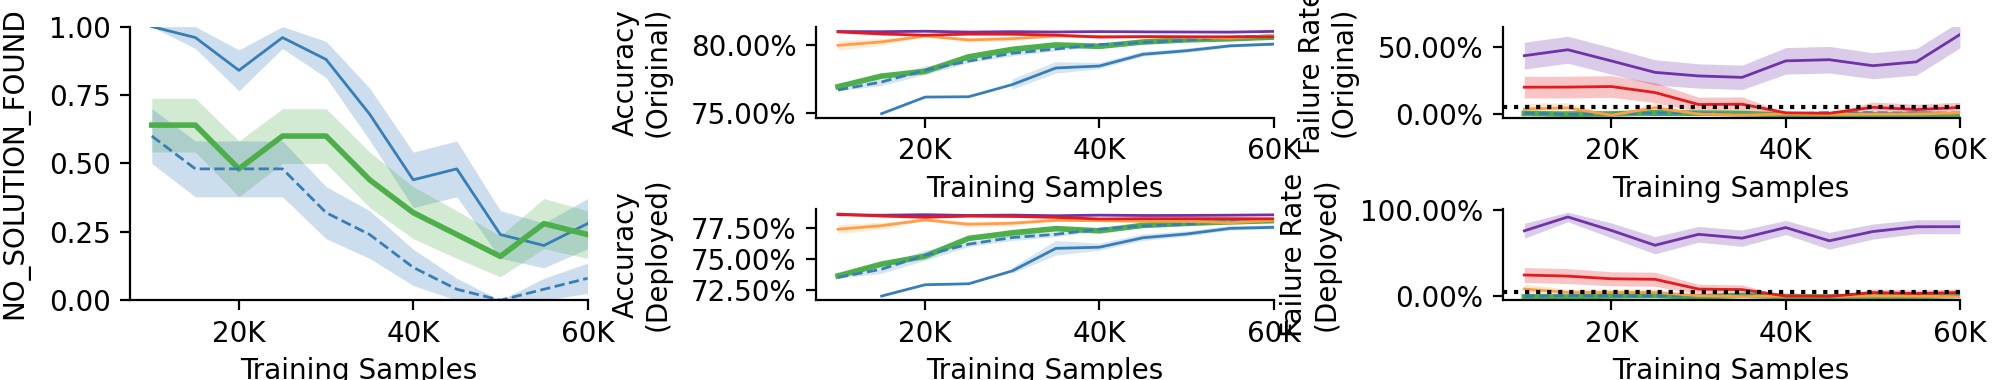
\includegraphics[width=\textwidth]{img/charts/adult/fixed/iclr_adult_demographic_shift_sex_eodds.png}
        \caption{Equalized Odds}
    \end{subfigure} 
    \begin{subfigure}[b]{1\linewidth}
        \includegraphics[width=\textwidth]{img/charts/adult/fixed/iclr_adult_demographic_shift_sex_pe.png}
        \caption{Predictive Equality}
    \end{subfigure} 
    \begin{subfigure}[b]{1\linewidth}
        \includegraphics[width=\textwidth]{img/charts/iclr_legend.png}
    \end{subfigure}
    \caption{Additional results when enforcing fairness constraints under known demographic shift
using the UCI Adult Census dataset.
}
\end{figure*}
\clearpage
\begin{figure}[h]
    \begin{subfigure}[b]{1\linewidth}
        \includegraphics[width=\textwidth]{img/charts/adult/antag/iclr_adult_demographic_shift_sex_di.png}
        \caption{Disparate Impact}
    \end{subfigure} 
    \begin{subfigure}[b]{1\linewidth}
        \includegraphics[width=\textwidth]{img/charts/adult/antag/iclr_adult_demographic_shift_sex_dp.png}
        \caption{Demographic Parity}
    \end{subfigure}
    \begin{subfigure}[b]{1\linewidth}
        \includegraphics[width=\textwidth]{img/charts/adult/antag/iclr_adult_demographic_shift_sex_eo.png}
        \caption{Equal Opportunity}
    \end{subfigure} 
    \begin{subfigure}[b]{1\linewidth}
        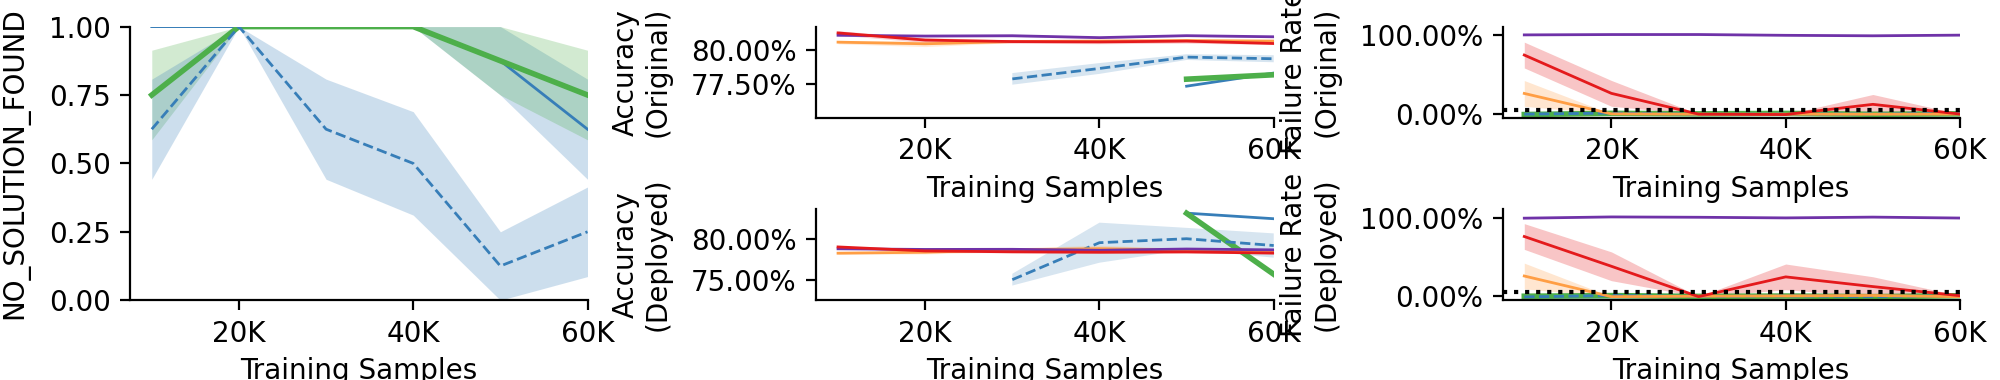
\includegraphics[width=\textwidth]{img/charts/adult/antag/iclr_adult_demographic_shift_sex_eodds.png}
        \caption{Equalized Odds}
    \end{subfigure} 
    \begin{subfigure}[b]{1\linewidth}
        \includegraphics[width=\textwidth]{img/charts/adult/antag/iclr_adult_demographic_shift_sex_pe.png}
        \caption{Predictive Equality}
    \end{subfigure} 
   \begin{subfigure}[b]{1\linewidth}
        \includegraphics[width=\textwidth]{img/charts/iclr_legend.png}
    \end{subfigure} 
    \caption{Additional results when enforcing fairness constraints under unknown demographic shift
using the UCI Adult Census dataset.
}
\end{figure}

\clearpage
\subsection{Brazil Dataset}
\begin{table}[H]
\begin{threeparttable}
\centering
\begin{tabular}{lrrrrrrrr}
\toprule
 & \multicolumn{4}{c}{Known DS} & \multicolumn{4}{c}{Unknown DS} \\
 & NSF & Acc & FR & $\Delta$ Acc & NSF & Acc & FR & $\Delta$ Acc \\
\cmidrule(r){2-5} \cmidrule{6-9}
FairConst & n/a & 0.612 & 1.000 & -0.000 & n/a & 0.612 & 1.000 & 0.000 \\
RFLearn & n/a & 0.648 & \bfseries 0.000 & 0.001 & n/a & 0.645 & \bfseries 0.000 & 0.000 \\
Fairlearn & n/a & 0.653 & 0.400 & 0.001 & n/a & 0.649 & 0.500 & 0.001 \\
Quasi-SC & 0.000 & \bfseries 0.657 & 0.160 & 0.006 & 0.000 & 0.655 & 0.050 & 0.007 \\
Shifty & 0.520 & 0.643\tnote{1} & \bfseries 0.000 & 0.058 & 0.800 & 0.628\tnote{2} & \bfseries 0.000 & n/a \\
SC & 0.000 & 0.656 & 0.080 & 0.005 & 0.000 & \bfseries 0.656 & 0.050 & 0.006 \\
\bottomrule
\end{tabular}
\begin{tablenotes}
\item[1] significantly worse than best model, $p<0.001$, $t=5.743$, $df=35$
\item[2] significantly worse than best model, $p=0.003$, $t=3.406$, $df=22$
\end{tablenotes}
\end{threeparttable}
\caption{Comparison between the models for the greatest sample size using the Demographic Parity fairness definition and Brazil dataset. When the \textit{DS} is known, Shifty differs significantly from the best performing model. There is no significant difference when the \textit{DS} is unknown.}
\label{dp_brazil}
\end{table}
\begin{table}[H]
\begin{threeparttable}
\centering
\begin{tabular}{lrrrrrrrr}
\toprule
 & \multicolumn{4}{c}{Known DS} & \multicolumn{4}{c}{Unknown DS} \\
 & NSF & Acc & FR & $\Delta$ Acc & NSF & Acc & FR & $\Delta$ Acc \\
\cmidrule(r){2-5} \cmidrule{6-9}
FairConst & n/a & 0.612 & 1.000 & -0.001 & n/a & 0.612 & 1.000 & 0.001 \\
RFLearn & n/a & 0.650 & \bfseries 0.000 & -0.001 & n/a & \bfseries 0.656 & 0.900 & 0.001 \\
Fairlearn & n/a & \bfseries 0.651 & 0.520 & -0.000 & n/a & 0.647 & 0.475 & 0.000 \\
Quasi-SC & 0.000 & 0.648 & 0.080 & 0.084 & 0.050 & 0.650 & 0.211 & 0.064 \\
Shifty & 0.920 & 0.570\tnote{1} & \bfseries 0.000 & n/a & 1.000 & n/a\tnote{2} & n/a & n/a \\
SC & 0.240 & 0.634 & \bfseries 0.000 & 0.108 & 0.350 & 0.640 & \bfseries 0.077 & 0.075 \\
\bottomrule
\end{tabular}
\begin{tablenotes}
\item[1] insufficient number of solutions to perform t-test
\item[2] insufficient number of solutions to perform t-test
\end{tablenotes}
\end{threeparttable}
\caption{Comparison between the models for the greatest sample size using the Equalized Odds fairness definition and Brazil dataset.}
\label{eodds_brazil}
\end{table}
\begin{table}[H]
\begin{threeparttable}
\centering
\begin{tabular}{lrrrrrrrr}
\toprule
 & \multicolumn{4}{c}{Known DS} & \multicolumn{4}{c}{Unknown DS} \\
 & NSF & Acc & FR & $\Delta$ Acc & NSF & Acc & FR & $\Delta$ Acc \\
\cmidrule(r){2-5} \cmidrule{6-9}
FairConst & n/a & 0.612 & 1.000 & -0.000 & n/a & 0.614 & 1.000 & 0.002 \\
RFLearn & n/a & 0.650 & 0.320 & 0.002 & n/a & 0.647 & 1.000 & 0.000 \\
Fairlearn & n/a & 0.651 & 0.400 & 0.000 & n/a & 0.648 & 0.550 & 0.002 \\
Quasi-SC & 0.000 & 0.655 & 0.040 & 0.110 & 0.050 & \bfseries 0.665 & 0.895 & 0.125 \\
Shifty & 0.960 & 0.532\tnote{1} & \bfseries 0.000 & -0.084 & 0.900 & 0.493\tnote{2} & \bfseries 0.000 & n/a \\
SC & 0.040 & \bfseries 0.657 & 0.042 & 0.130 & 0.150 & 0.663 & 0.882 & 0.239 \\
\bottomrule
\end{tabular}
\begin{tablenotes}
\item[1] insufficient number of solutions to perform t-test
\item[2] insufficient number of solutions to perform t-test
\end{tablenotes}
\end{threeparttable}
\caption{Comparison between the models for the greatest sample size using the Equal Opportunity fairness definition and Brazil dataset.}
\label{eopp_brazil}
\end{table}


\begin{table}[H]
\begin{threeparttable}
\centering
\begin{tabular}{lrrrrrrrr}
\toprule
 & \multicolumn{4}{c}{Known DS} & \multicolumn{4}{c}{Unknown DS} \\
 & NSF & Acc & FR & $\Delta$ Acc & NSF & Acc & FR & $\Delta$ Acc \\
\cmidrule(r){2-5} \cmidrule{6-9}
FairConst & n/a & 0.613 & 1.000 & 0.000 & n/a & 0.612 & 1.000 & 0.000 \\
RFLearn & n/a & 0.649 & 0.440 & 0.001 & n/a & 0.648 & 0.150 & -0.001 \\
Fairlearn & n/a & 0.650 & 0.900 & 0.000 & n/a & 0.648 & 0.925 & -0.000 \\
Quasi-SC & 0.000 & \bfseries 0.657 & 0.680 & 0.025 & 0.000 & 0.656 & 0.400 & 0.014 \\
Shifty & 0.880 & 0.618\tnote{1} & \bfseries 0.000 & -0.009 & 0.850 & 0.629\tnote{2} & \bfseries 0.000 & -0.011 \\
SC & 0.040 & 0.656 & 0.375 & 0.129 & 0.200 & \bfseries 0.658 & \bfseries 0.000 & 0.092 \\
\bottomrule
\end{tabular}
\begin{tablenotes}
\item[1] significantly worse than best model, $p<0.001$, $t=6.943$, $df=26$
\item[2] significantly worse than best model, $p=0.008$, $t=2.981$, $df=17$
\end{tablenotes}
\end{threeparttable}
\caption{Comparison between the models for the greatest sample size using the Predictive Equality fairness definition and Brazil dataset. Shifty performs significantly worse than the best model for both the known and unknown demographic shift.}
\label{pe_brazil}
\end{table}

\begin{figure*}[h]
    \begin{subfigure}[b]{1\linewidth}
        \includegraphics[width=\textwidth]{img/charts/brazil/fixed/iclr_brazil_demographic_shift_sex_di.png}
        \caption{Disparate Impact}
    \end{subfigure} 
    \begin{subfigure}[b]{1\linewidth}
        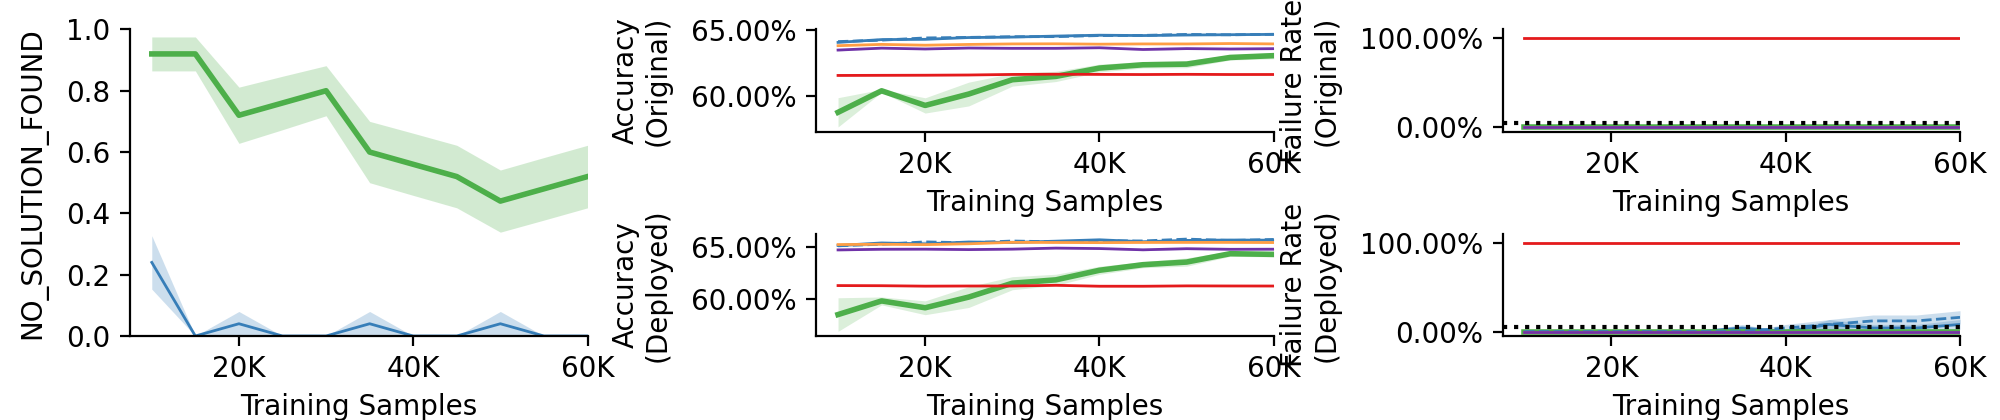
\includegraphics[width=\textwidth]{img/charts/brazil/fixed/iclr_brazil_demographic_shift_sex_dp.png}
        \caption{Demographic Parity}
    \end{subfigure}
    \begin{subfigure}[b]{1\linewidth}
        \includegraphics[width=\textwidth]{img/charts/brazil/fixed/iclr_brazil_demographic_shift_sex_eo.png}
        \caption{Equal Opportunity}
    \end{subfigure} 
    \begin{subfigure}[b]{1\linewidth}
        \includegraphics[width=\textwidth]{img/charts/brazil/fixed/iclr_brazil_demographic_shift_sex_eodds.png}
        \caption{Equalized Odds}
    \end{subfigure} 
    \begin{subfigure}[b]{1\linewidth}
        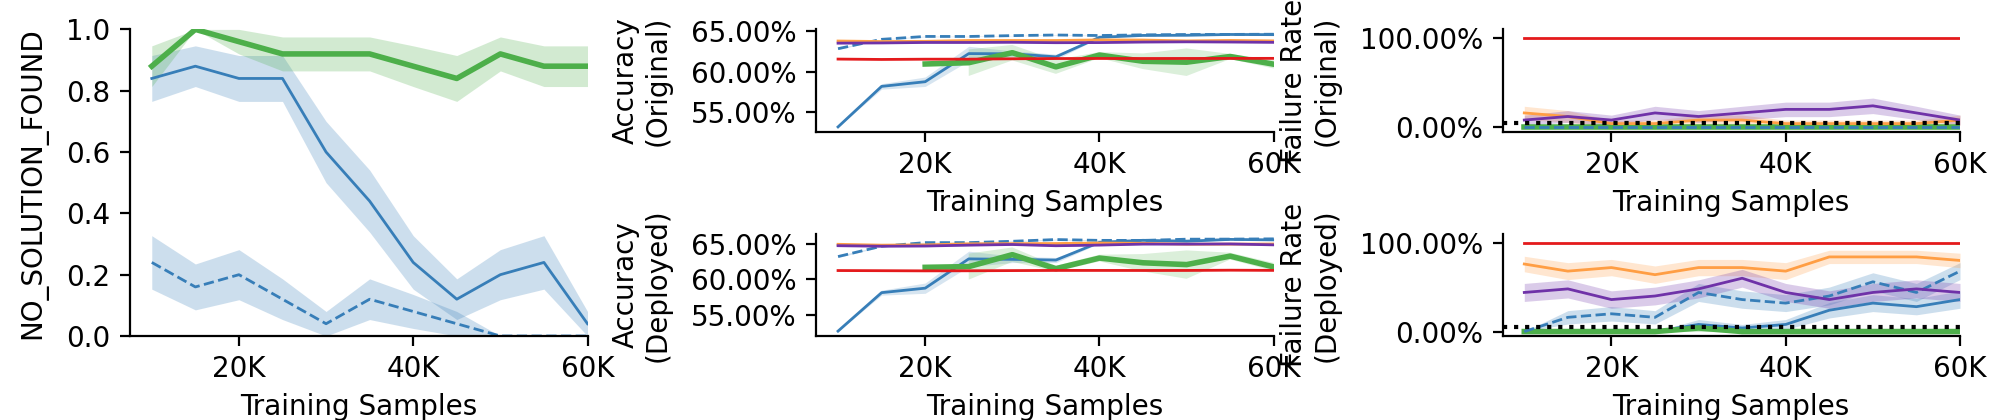
\includegraphics[width=\textwidth]{img/charts/brazil/fixed/iclr_brazil_demographic_shift_sex_pe.png}
        \caption{Predictive Equality}
    \end{subfigure} 
    \begin{subfigure}[b]{1\linewidth}
        \includegraphics[width=\textwidth]{img/charts/iclr_legend.png}
    \end{subfigure}
    \caption{Additional results when enforcing fairness constraints under known demographic shift
using the UFRGS Entrance Exam and GPA dataset.
}
\end{figure*}

\begin{figure}[h]
    \begin{subfigure}[b]{1\linewidth}
        \includegraphics[width=\textwidth]{img/charts/brazil/antag/iclr_brazil_demographic_shift_sex_di.png}
        \caption{Disparate Impact}
    \end{subfigure} 
    \begin{subfigure}[b]{1\linewidth}
        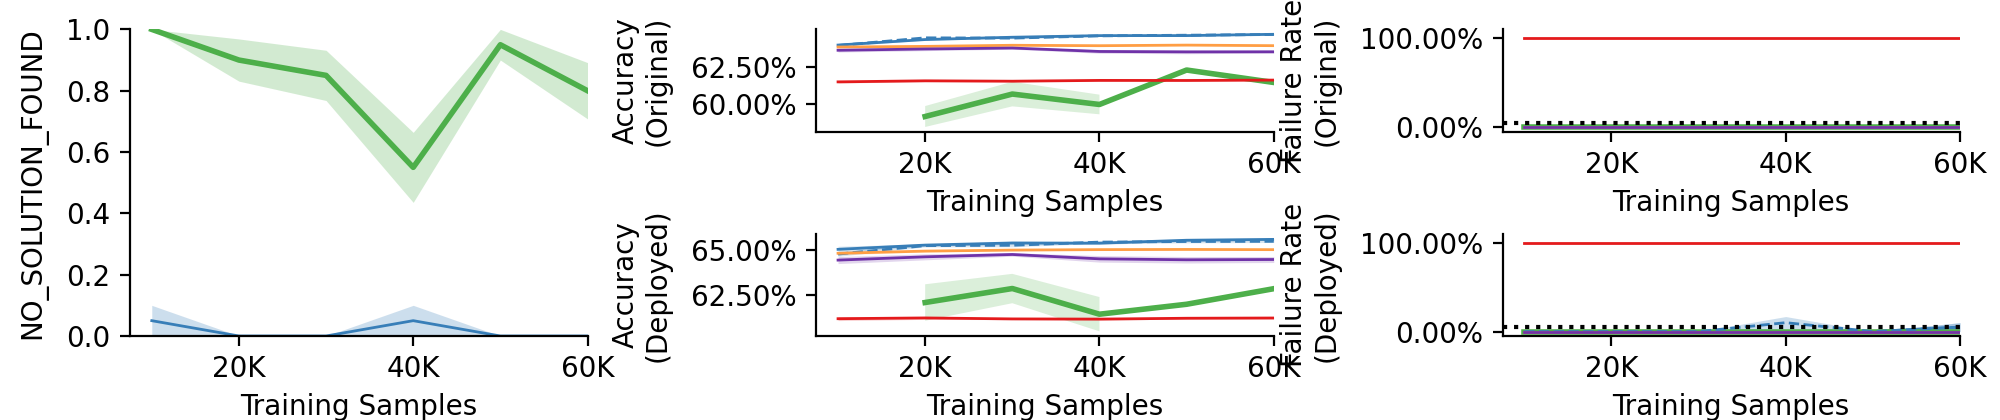
\includegraphics[width=\textwidth]{img/charts/brazil/antag/iclr_brazil_demographic_shift_sex_dp.png}
        \caption{Demographic Parity}
    \end{subfigure}
    \begin{subfigure}[b]{1\linewidth}
        \includegraphics[width=\textwidth]{img/charts/brazil/antag/iclr_brazil_demographic_shift_sex_eo.png}
        \caption{Equal Opportunity}
    \end{subfigure} 
    \begin{subfigure}[b]{1\linewidth}
        \includegraphics[width=\textwidth]{img/charts/brazil/antag/iclr_brazil_demographic_shift_sex_eodds.png}
        \caption{Equalized Odds}
    \end{subfigure} 
    \begin{subfigure}[b]{1\linewidth}
        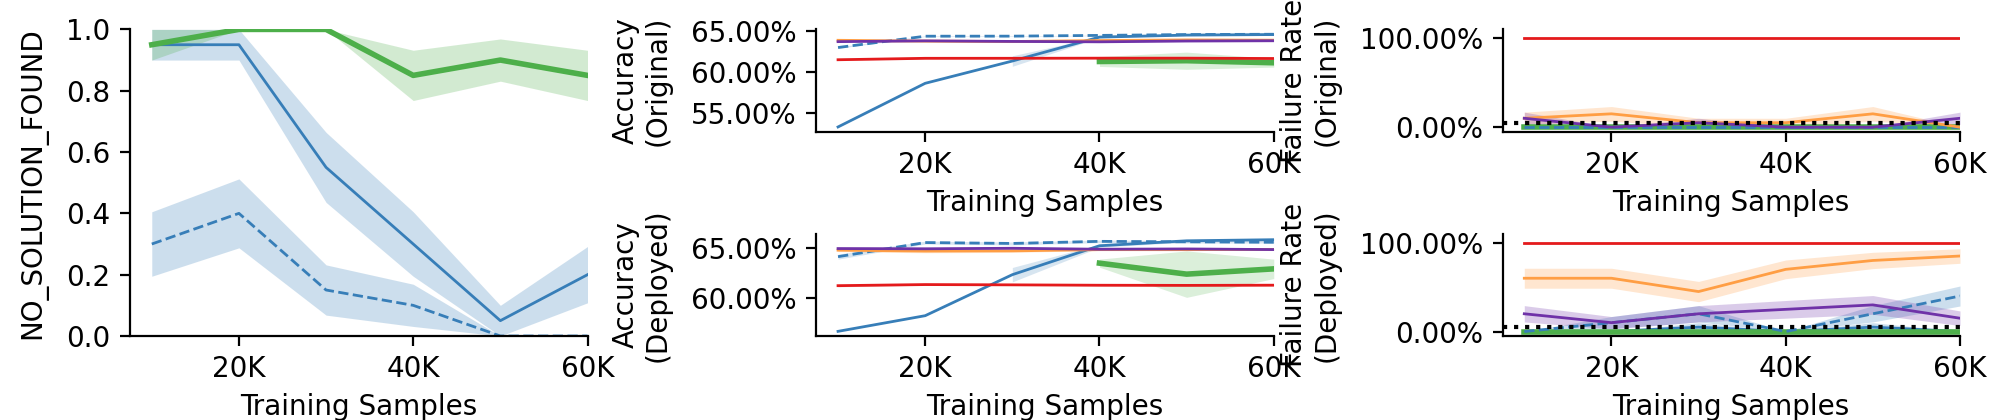
\includegraphics[width=\textwidth]{img/charts/brazil/antag/iclr_brazil_demographic_shift_sex_pe.png}
        \caption{Predictive Equality}
    \end{subfigure} 
   \begin{subfigure}[b]{1\linewidth}
        \includegraphics[width=\textwidth]{img/charts/iclr_legend.png}
    \end{subfigure} 
    \caption{Additional results when enforcing fairness constraints under unknown demographic shift
using the UFRGS Entrance Exam and GPA dataset.
}
\end{figure}
\clearpage

\subsection{Additional results beyond original paper}
\label{add_beyond}

 
\begin{table}[H]
\centering
\label{di_brazil_optimizer}
\begin{tabular}{lrrrrrrrr}
\toprule
 & \multicolumn{4}{c}{Known DS} & \multicolumn{4}{c}{Unknown DS} \\
 & NSF & Acc & FR & $\Delta$ Acc & NSF & Acc & FR & $\Delta$ Acc \\
\cmidrule(r){2-5} \cmidrule{6-9}
CMA-ES & 0.600 & \bfseries 0.606 & \bfseries 0.000 & 0.130 & 0.450 & \bfseries 0.480 & \bfseries 0.000 & 0.030 \\
BFGS & 0.440 & 0.596 & \bfseries 0.000 & 0.120 & 0.050 & 0.469 & \bfseries 0.000 & 0.019 \\
\bottomrule
\end{tabular}
\caption{Comparison between CMA-ES and BFGS optimization methods for the \textit{Shifty} implementation using the Brazil dataset and the Disparate Impact fairness definition.}
\end{table}

\begin{table}[H]
\centering
\label{dp_adult_optimizer}
\begin{tabular}{lrrrrrrrr}
\toprule
 & \multicolumn{4}{c}{Known DS} & \multicolumn{4}{c}{Unknown DS} \\
 & NSF & Acc & FR & $\Delta$ Acc & NSF & Acc & FR & $\Delta$ Acc \\
\cmidrule(r){2-5} \cmidrule{6-9}
CMA-ES & 0.480 & \bfseries 0.756 & \bfseries 0.000 & 0.020 & 0.000 & \bfseries 0.780 & \bfseries 0.000 & 0.020 \\
BFGS & 0.240 & 0.731 & \bfseries 0.000 & 0.014 & 0.100 & 0.755 & \bfseries 0.000 & 0.016 \\
\bottomrule
\end{tabular}
\caption{Comparison between CMA-ES and BFGS optimization methods for the \textit{Shifty} implementation using the UCI Adult Census dataset and the Demographic Parity fairness definition.}
\end{table}
 
\begin{table}[H]
\centering
\label{dp_brazil_optimizer}
\begin{tabular}{lrrrrrrrr}
\toprule
 & \multicolumn{4}{c}{Known DS} & \multicolumn{4}{c}{Unknown DS} \\
 & NSF & Acc & FR & $\Delta$ Acc & NSF & Acc & FR & $\Delta$ Acc \\
\cmidrule(r){2-5} \cmidrule{6-9}
CMA-ES & 0.520 & \bfseries 0.643 & \bfseries 0.000 & 0.058 & 0.800 & \bfseries 0.628 & \bfseries 0.000 & n/a \\
BFGS & 0.480 & 0.638 & \bfseries 0.000 & 0.079 & 0.600 & 0.613 & \bfseries 0.000 & 0.034 \\
\bottomrule
\end{tabular}
\caption{Comparison between CMA-ES and BFGS optimization methods for the \textit{Shifty} implementation using the Brazil dataset and the Demographic Parity fairness definition.}
\end{table}
